\chapter{EXTRAÇÃO DE PONTOS DE FORMA AUTOMÁTICA} \label{cha:introd} 

Neste capítulo, será apresentado o método de extração automática de pontos de forma a facilitar a modelagem de \textit{splines} para reconhecimento facial. O método proposto consiste em um algoritmo que utiliza técnicas de processamento de imagem e otimização para extrair pontos relevantes em imagens faciais. A abordagem é baseada na detecção de características faciais, seguida pela extração de contornos e filtragem dos pontos obtidos.

Inicialmente, realizamos uma pesquisa para identificar as principais características faciais a serem extraídas, decidindo focar na detecção dos olhos, nariz e boca. Para isso, utilizamos o algoritmo Haar Cascade para detectar o rosto da pessoa na imagem, concentrando a análise nessa área específica e facilitando a detecção das características menores \cite{BoostedCascade}.

Em seguida, utilizamos o método \texttt{Canny} do OpenCV \cite{CannyAplicacao} para extrair os contornos das características faciais. O \texttt{Canny} é um algoritmo de detecção de contornos eficiente que nos ajuda a identificar os limites das características faciais com maior precisão \cite{Canny}.

Após a extração dos contornos, suprimimos alguns pontos fazendo o uso de grafos e árvores geradoras mínimas. Essa etapa é crucial para reduzir a quantidade de pontos a serem utilizados na modelagem das \textit{splines}, mantendo apenas os pontos mais significativos que representam as características faciais. A simplificação dos pontos é realizada utilizando o algoritmo construído de forma autoral e implementado em Python, que utiliza a biblioteca \textit{Scipy} \cite{Scipy} para encontrar a árvore geradora mínima. Essa abordagem garante que os pontos extraídos sejam representativos e relevantes para a modelagem das \textit{splines}.

Por fim, ainda é possível aplicar um filtro de suavização para diminuir a quantidade de pontos, fazendo isso de forma completamente aleatória, mantendo apenas os pontos iniciais e finais de cada segmento, o que pode ser útil para melhorar a qualidade da modelagem das \textit{splines}.

\section{MODELOS PARA DETECÇÃO DE CARACTERÍSTICAS}

Foi utilizada uma abordagem popular de detecção chamada Haar Cascade, implementada com OpenCV e Python. Este método, introduzido e estudado no artigo \cite{BoostedCascade}, permite a detecção eficaz das características faciais.

O classificador Haar Cascade já foi calibrado e validado com um vasto conjunto de dados de rostos humanos, eliminando a necessidade de calibração adicional. Basta carregar o classificador da biblioteca e utilizá-lo para detectar rostos em uma imagem de entrada.

Para distinguir com precisão entre amostras que contêm ou não um rosto humano, utilizamos um classificador forte, resultante da combinação de diversos classificadores. Esta técnica envolve a utilização de uma cascata de classificadores para identificar diferentes características em uma imagem.

Os seguintes classificadores foram utilizados:

\begin{itemize}
    \item \texttt{haarcascade\_frontalface\_default.xml}
    \item \texttt{haarcascade\_eye.xml}
    \item \texttt{haarcascade\_mcs\_nose.xml}
    \item \texttt{haarcascade\_mcs\_mouth.xml}
\end{itemize}

Todos os classificadores mencionados podem ser encontrados no repositório do OpenCV no GitHub \cite{HaarAplicacao}.

\subsection{Parâmetros}

Após carregar os classificadores, podemos utilizá-los aplicando quatro parâmetros específicos para cada um.

O método \texttt{detectMultiScale()} é utilizado para identificar faces de diferentes tamanhos na imagem de entrada. Os quatro parâmetros principais deste método são detalhados a seguir:

\begin{itemize}
    \item \textbf{\texttt{image}}:
    \begin{itemize}
    \item O primeiro parâmetro é a imagem em tons de cinza. Essa imagem serve como entrada para o método e com ela em tons de cinza facilita a detecção de características faciais.
    \end{itemize}

\item \textbf{\texttt{scaleFactor}}:
\begin{itemize}
    \item Este parâmetro é usado para reduzir o tamanho da imagem de entrada, facilitando a detecção de faces maiores pelo algoritmo. Especificamos um fator de escala de 1.1, indicando que queremos reduzir o tamanho da imagem em 10\%.
    \end{itemize}

\item \textbf{\texttt{minNeighbors}}:
\begin{itemize}
    \item O classificador em cascata aplica uma janela deslizante através da imagem para detectar faces. Essas janelas são representadas como retângulos. Inicialmente, o classificador captura um grande número de falsos positivos. O parâmetro \texttt{minNeighbors} especifica o número de retângulos vizinhos que precisam ser identificados para que um objeto seja considerado uma detecção válida, ou seja, valores pequenos como 0 ou 1 resultam em muitos falsos positivos, enquanto valores grandes podem levar à perda de verdadeiros positivos. É necessário encontrar um equilíbrio que elimine falsos positivos e identifique com precisão os verdadeiros positivos.
\end{itemize}

\item \textbf{\texttt{minSize}}:
\begin{itemize}
    \item Este parâmetro define o tamanho mínimo do objeto a ser detectado. O modelo ignorará faces menores do que o tamanho mínimo especificado.
\end{itemize}

\end{itemize}

Foi colocado como default para todos os classificadores os seguintes valores: 

{\small \texttt{detectMultiScale(image, scaleFactor=1.1, minNeighbors=5, minSize=(40, 50))}}

\subsection{Resultado da Detecção das Características}

Para realizar a detecção das características faciais, inicialmente identificamos o rosto na imagem. Este processo retorna um \textit{array} com quatro valores: as coordenadas $x$ e $y$ do ponto onde o rosto foi detectado, além de sua largura e altura. Em seguida, recortamos a imagem nessa região, de modo a isolar a face da pessoa.

Com o rosto isolado, aplicamos classificadores específicos para detectar o nariz, a boca e os olhos.

Essa abordagem, que realiza a detecção passo a passo, garante maior precisão na identificação das características menores, pois concentra a análise na área previamente delimitada pelo rosto.

Como exemplo, considere a \autoref{fig:rosto} e a \autoref{fig:caracteristicas} , onde a sequência de detecção é ilustrada:

\begin{enumerate}
\item \textbf{Detecção do Rosto:} Para identificar e isolar o rosto na imagem usamos o classificador \texttt{haarcascade\_frontalface\_default.xml}.
\item \textbf{Detecção dos Olhos:} Aplicamos o classificador \texttt{haarcascade\_eye.xml} para localizar os olhos dentro da área do rosto previamente detectada.
\item \textbf{Detecção do Nariz:} Utilizamos o classificador \texttt{haarcascade\_mcs\_nose.xml} para identificar o nariz na mesma área delimitada.
\item \textbf{Detecção da Boca:} Finalmente, aplicamos o classificador 

\texttt{haarcascade\_mcs\_mouth.xml} para localizar a boca.
\end{enumerate}

% \imagem{Exemplo de detecção do rosto}{\includegraphics[width = 80mm]{fig/face}}{}{rosto}{}{}
% \imagem{Exemplo de detecção das características faciais}{\includegraphics[width = 80mm]{fig/caracteristicas}}{}{caracteristicas}{}{}



\section{Extração de Contornos}

A detecção de bordas é essencial para a análise de imagens, pois permite a identificação de contornos e a segmentação de objetos em uma cena. O algoritmo \cite{Canny} é um dos métodos mais populares devido à sua eficiência e precisão. Esta parte irá explorar o funcionamento do algoritmo de Canny e demonstrará sua aplicação prática com a biblioteca OpenCV \cite{CannyAplicacao}.

\subsection{Algoritmo de Canny}

O algoritmo de detecção de bordas de Canny é composto por várias etapas, conforme descrito a seguir:

\begin{enumerate}
    \item \textbf{Redução de Ruído}: A imagem é suavizada com um filtro Gaussiano para minimizar a interferência do ruído na detecção de bordas.

    \item \textbf{Cálculo do Gradiente de Intensidade}: Os gradientes de intensidade são calculados nas direções horizontal \(G_x\) e vertical \(G_y\) usando operadores Sobel. A mag   nitude do gradiente é dada por:
    \[G_x = \frac{\partial I}{\partial x} \quad G_y = \frac{\partial I}{\partial y}\]
    \[Borda\_Gradiente(G) = \sqrt{G_{x}^{2} + G_{y}^{2}}\]

    \item \textbf{Supressão Não Máxima}: Elimina \textit{pixels} que não são máximos locais no gradiente, preservando apenas os que representam bordas fortes.

    \item \textbf{Rastreamento de Bordas por Histerese}: Classifica as bordas detectadas usando dois limiares, \textit{minVal} e \textit{maxVal}:
    \begin{itemize}
        \item Bordas com gradiente maior que \textit{maxVal} são fortes.
        \item Bordas com gradiente menor que \textit{minVal} são descartadas.
        \item Bordas entre \textit{minVal} e \textit{maxVal} são fracas e mantidas apenas se conectadas a bordas fortes.
    \end{itemize}
\end{enumerate}

Por exemplo, na Figura \autoref{fig:histerese}, a borda A está acima do \textit{maxVal}, sendo assim considerada uma \textit{sure-edge}. Embora a borda C esteja abaixo do \textit{maxVal}, ela está conectada à borda A, de modo que também é considerada como borda válida, resultando em uma curva completa. Já a borda B, embora esteja acima do \textit{minVal}, não está conectada a nenhuma \textit{sure-edge} e, portanto, é descartada.

\imagem{Rastreamento de contorno por histerese}{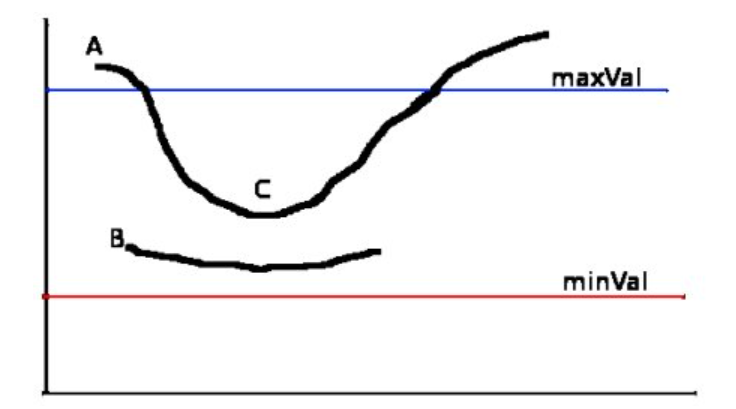
\includegraphics[width = 80mm]{fig/histerese}}{\cite{CannyAplicacao}}{histerese}{}{Calculada a magnitude do gradiente ao longo de uma curva parametrizada.}

É crucial selecionar adequadamente os valores de \textit{minVal} e \textit{maxVal} para obter resultados precisos. Esse estágio também ajuda a remover pequenos ruídos de pixels, assumindo que as bordas são linhas longas e contínuas.

\section{Resultado da Detecção de Bordas}
\label{sec:resultado-deteccao-bordas}

Ao aplicar o algoritmo de Canny para a detecção de bordas, obtemos um array binário onde os valores '0' e '255' representam diferentes tipos de pixels. Os pixels com valor '0' são considerados descartáveis, ou seja, não fazem parte das bordas detectadas. Em contraste, os pixels com valor '255' são os que definem as bordas, indicando regiões de mudança de intensidade significativa na imagem original.

A seguir são apresentados os resultados da aplicação do algoritmo de Canny em imagens de exemplo. As Figuras ,  e mostram as imagens originais e as imagens com as bordas detectadas.



